\pgfplotsset{compat=1.3,
    %legend drawing style, single bar instead of the default double mini bars
    /pgfplots/ybar legend/.append style={
        /pgfplots/legend image code/.code={%
           \draw[##1,/tikz/.cd,yshift=-0.25em]
           (0cm,0cm) rectangle (5pt,0.8em);
        },
    }
}

%%sharp linear plots
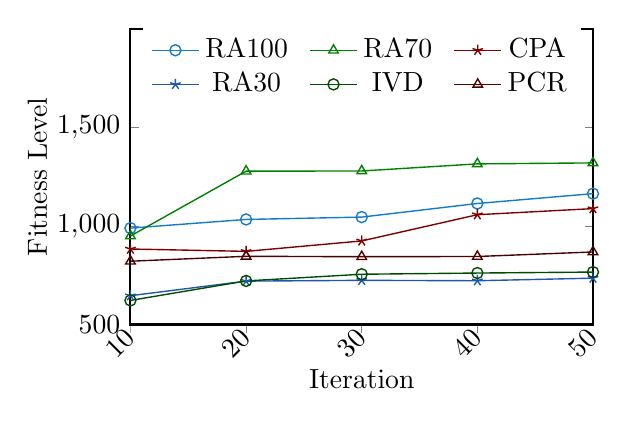
\begin{tikzpicture}
%remove space surrounding text nodes and the whole picture caused by text
%[every node/.style={inner sep=0,outer sep=0}]

%\pgfplotstableread{
%Iteration IVD\_IVD
%1       99.69	
%2       99.59	
%3       99.58	
%4       99.80	
%5       99.85	
%6       99.11	
%7       87.73	
%8       99.83	
%9       99.42
%10      99.68
%}\loadedtable

\pgfplotstableread{
Iteration RA100 RA70	CPA	RA30	IVD	PCR
1	989	949	883	646	622	821
2	1033	1278	871	720	721	846
3	1045	1279	924	724	755	844
4	1114	1315	1057	722	761	845
5	1164	1320	1088	735	766	868

}\loadedtable

\begin{axis}[
%xaxis styles
%xticklabels={s5378,s9234, s13207, s15850, s38584,systemcdes, mem\_ctrl, usb\_funct, ac97\_ctr, pci\_bridge32},
xticklabels={10, 20, 30, 40, 50},
xtick={1,...,5},
%x axis limits
xmin=1, xmax=5,
%x and y axes scaling
x=1.4685714cm, y=0.0025cm,
x tick label style={rotate=45, xshift=0pt,yshift=0pt,anchor=east,
%"inner sep" removes the space surrounding label tick texts at the bottom,
%so that there is no useless white space at the lower boundary of the picture. The
%space of tick label texts need to be removed because they are the lowest
%units without an xlable
inner sep=0},
xticklabel pos=left, xtick align=outside, xtick pos=left,
%
%y axis limits
ymin=500, ymax=2000,
%yaxis styles
ylabel={Fitness Level},
xlabel={Iteration},
%"inner sep" for ylabel removes the white space on the leftmost edge of the picture
ylabel style={inner sep=0},
ylabel shift=0pt, ytickmin=500,ytickmax=1500,
% ytick = {700,800,900,1000,1100,1200,1300}, yticklables = {700,800,900,1000,1100,1200,1300}
%
%legend styles
legend columns=3,
legend style={
at={(0.5,0.87)}, anchor=center,
%column separation between legend items
/tikz/every even column/.append style={column sep=0.2cm},
%distance between legend symbols and text nodes
%column sep=2.5cm,
%space surrounding the text boxes in legend
%nodes={inner xsep=20pt},
%no stroke in legend
draw=none,
},
%
%axis drawing line width
line width=0.75pt,
major tick length=3pt,
]  \addplot[sharp plot, line width=0.5pt, cyan!60!blue, mark=o, fill=none] table[x=Iteration,y=RA100] {\loadedtable};
\addplot[sharp plot, line width=0.5pt, green!50!black, mark=triangle, fill=none] table[x=Iteration,y=RA70] {\loadedtable};
\addplot[sharp plot, line width=0.5pt, red!50!black, mark=star, fill=none] table[x=Iteration,y=CPA] {\loadedtable};
\addplot[sharp plot, line width=0.5pt, cyan!30!blue, mark=star, fill=none] table[x=Iteration,y=RA30] {\loadedtable};
\addplot[sharp plot, line width=0.5pt, green!30!black, mark=o, fill=none] table[x=Iteration,y=IVD] {\loadedtable};
\addplot[sharp plot, line width=0.5pt, red!30!black, mark=triangle, fill=none] table[x=Iteration,y=PCR] {\loadedtable};
   %\addplot[sharp plot, line width=0.5pt, green!50!black, mark=triangle, fill=none] table[x=Iteration,y=tested] {\loadedtable};
   %\addplot[sharp plot, line width=0.5pt, red!50!black, mark=star, fill=none] table[x=Iteration,y=nobuffer] {\loadedtable};
\legend{RA100,RA70,CPA,RA30,IVD,PCR}
\end{axis}
\end{tikzpicture}
